\documentclass{beamer}
\usepackage[T1]{fontenc}
\usepackage[utf8]{inputenc}
\usepackage{lmodern}
\usepackage[polish]{babel}
\usepackage{graphicx}
\usepackage{multirow}

\usetheme{AGH}

\title[Interpolacja obrazu barwnego]{Równoległa interpolacja obrazu barwnego
  z~kamery cyfrowej}

\author[B. Bułat, T. Drzewiecki]{Bartłomiej Bułat, Tomasz Drzewiecki}

\date[2011]{24.01.2012}

\institute[AGH]
{Wydział EAIiIB\\ 
Katedra Automatyki i Inżynierii Biomedycznej
}

\setbeamertemplate{itemize item}{$\maltese$}

\begin{document}

{
\usebackgroundtemplate{
\includegraphics[width=\paperwidth]{titlepagepl}} % wersja polska
 \begin{frame}
   \titlepage
 \end{frame}
}

%---------------------------------------------------------------------------

%% Figure example
%\begin{figure}
%  \includegraphics[width=0.5\textwidth]{filename}
%  \caption{Figure caption}
%  \label{fig:label}
%\end{figure}

\begin{frame}
\frametitle{Wstęp}

\end{frame}

\begin{frame}
  \frametitle{Implementacja kontrollera po stronie CPU}
  W~celu łatwiejszej, szybszej oraz generującej mniej błędów implementacji stworzono maly framework klas realizujących obsługę OpenCL od strony procesora.
Schemat jego struktury jest przedstawiony na rys. \ref{fig:class_diagram} na następnym slajdzie.
\end{frame}

\begin{frame}
  \frametitle{Diagram klas}
\begin{figure}
  \centering
  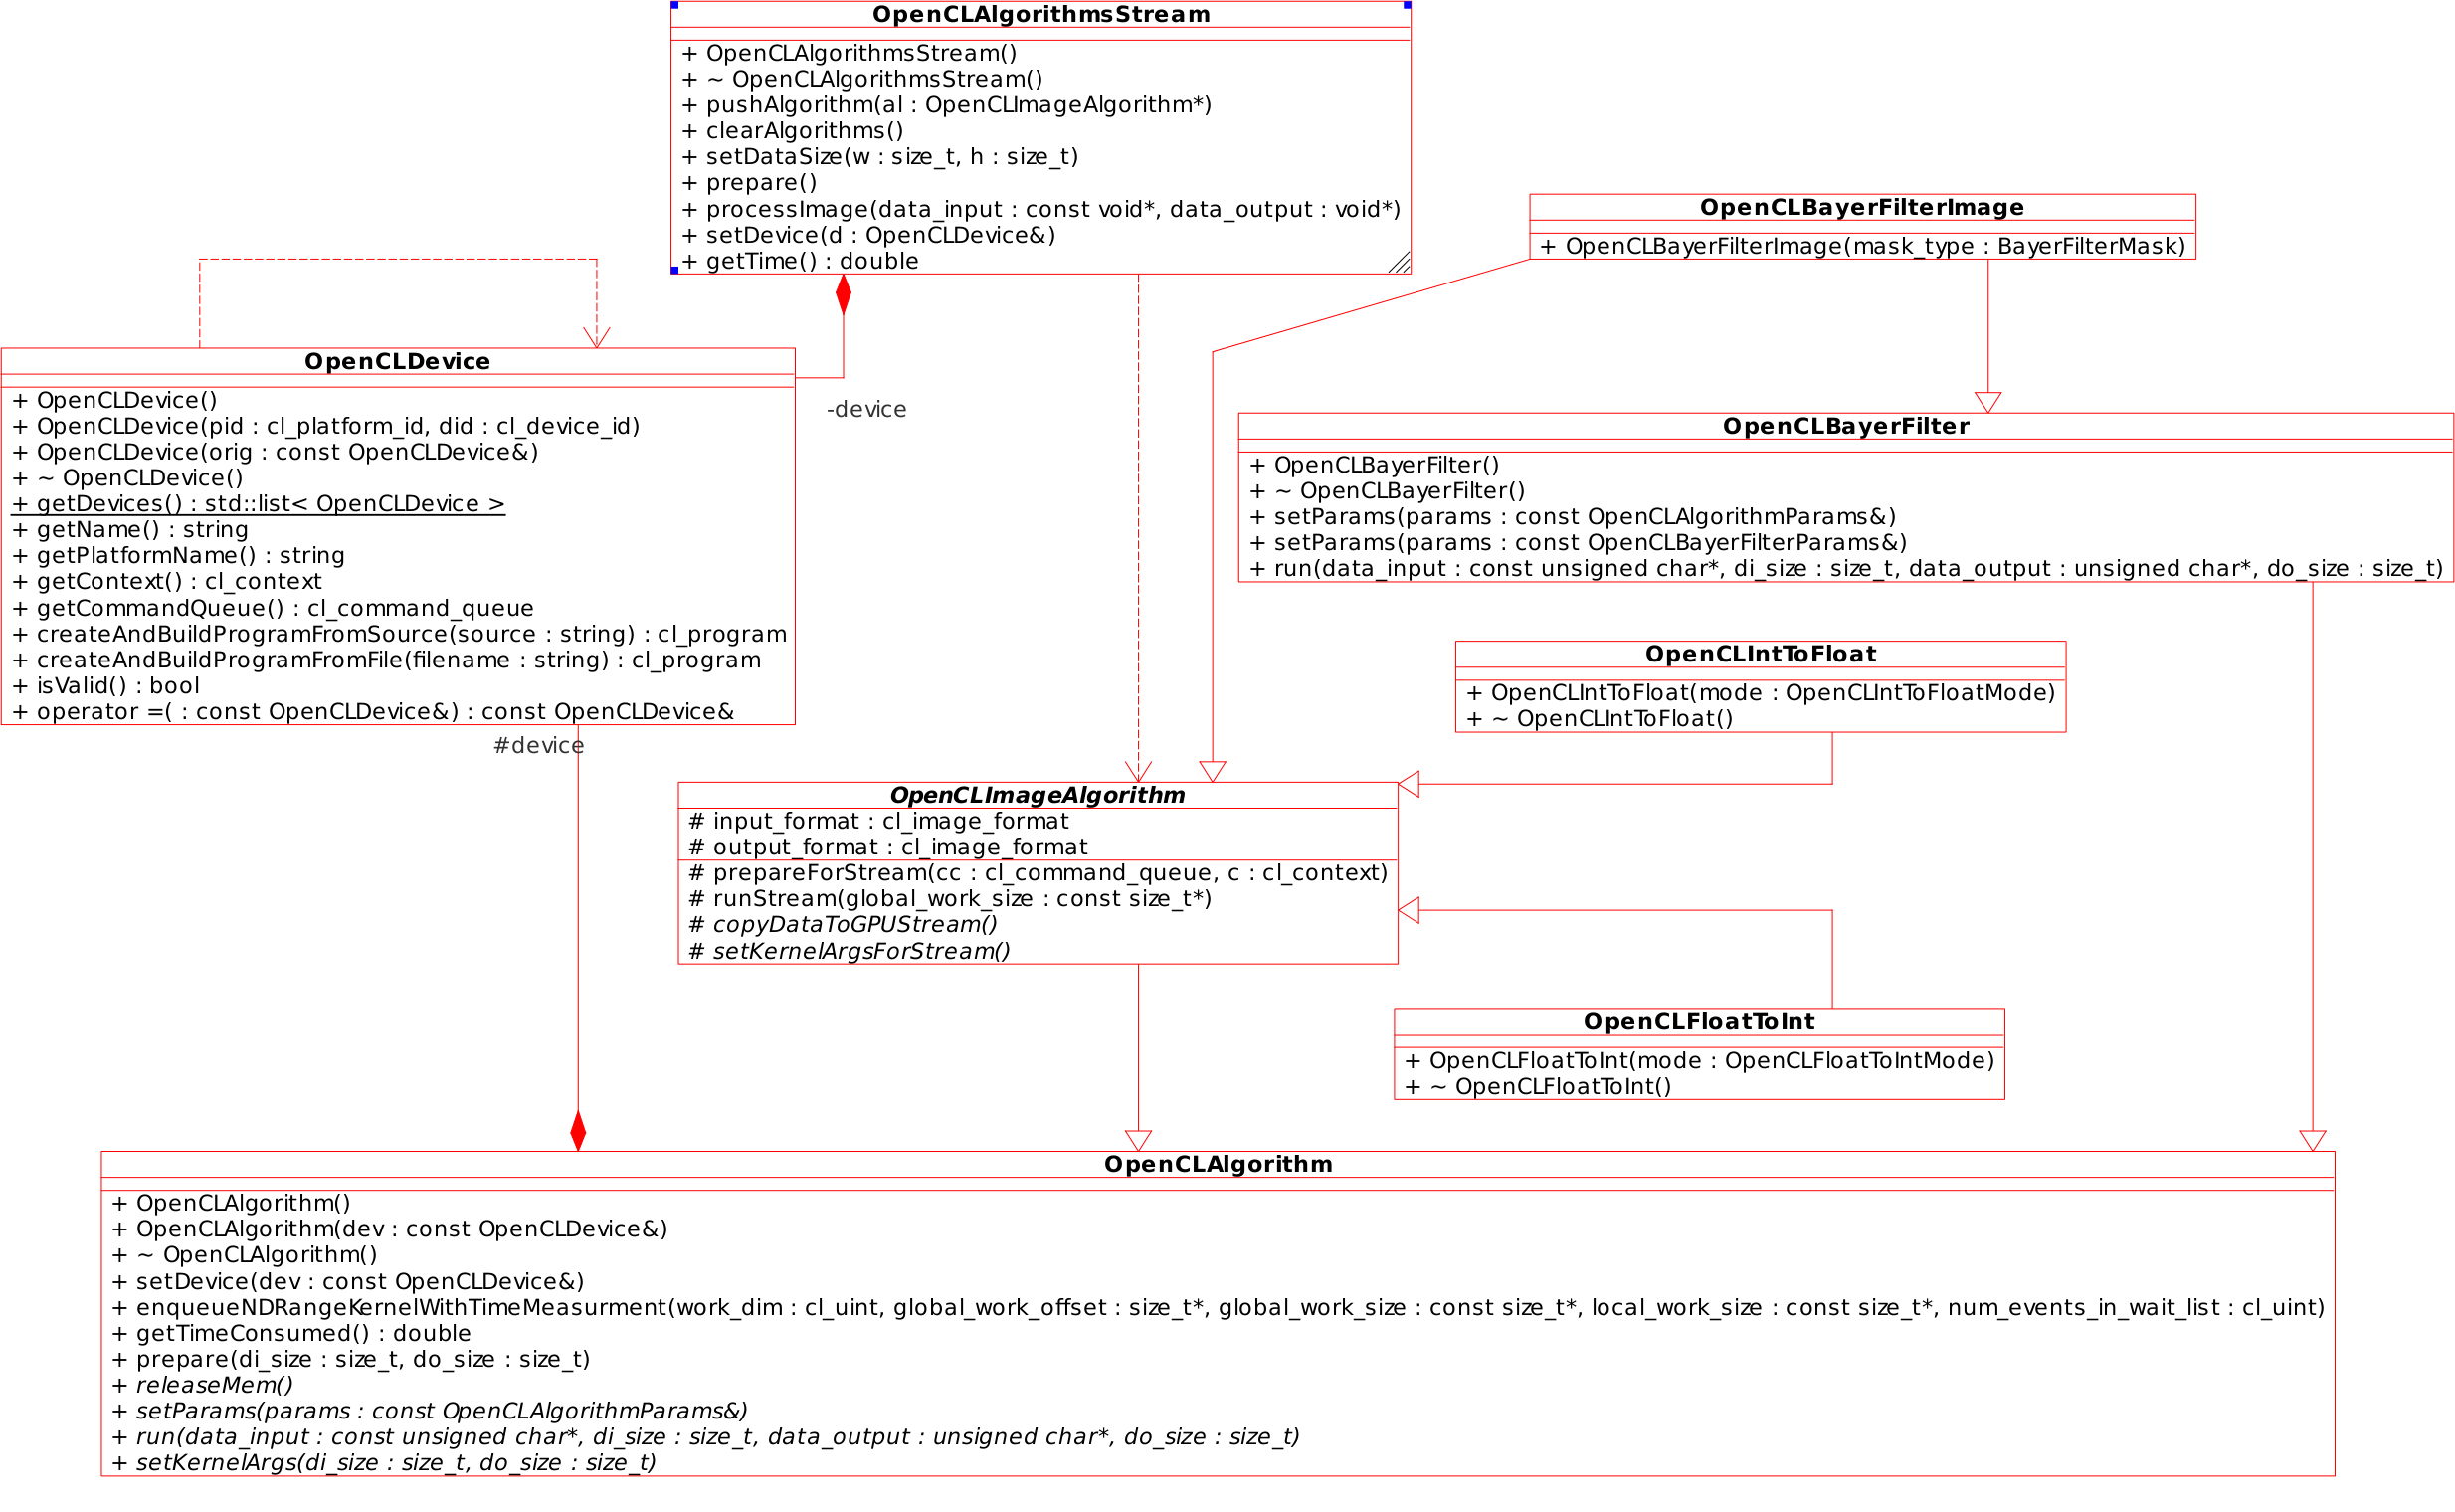
\includegraphics[width=0.6\linewidth]{class_diagram}
  \caption{Diagram klas stworzonego frameworku.}
  \label{fig:class_diagram}
\end{figure}
  
\end{frame}

\begin{frame}
  \frametitle{Testowanie - sprzęt}
  Testy algorytmu zostały zrealizowane z użyciem dwóch kart graficznych o~parametrach:
\begin{center}
\begin{table}
   \begin{tabular}{ |l | l | l | }
     \hline
       & GT 555M & GT9800 \\ \hline
     Liczba rdzeni & 144 & 128 \\ \hline
     Częstotliwość rdzenia & 1250MHz & 600MHz \\ \hline
     Częstotliwość pamięci & 1800MHz & 900MHz \\ \hline
     Magistrala pamięci & 128bit & 256bit \\ \hline

   \end{tabular}
  \caption{Porówanie kart graficznych użytych do testów.}
  \label{tab:gpus}
\end{table}
\end{center}
Do obliczeń referencyjnych użyto procesora Intel Core i7-2670QM 2,2GHz.
\end{frame}
\begin{frame}
  \frametitle{Testowanie - procedura}
  Algorytmy testowano na 79 obrazach o wymiarach 2546x2058 pikseli. Do każdego testu użyto tych samych obrazów, które były zapisane na dysku. Czas odczytywania obrazów z plików nie był doliczany do czasu obliczeń. Liczono czas wykonania wszystkich operacji koniecznych do wykonania algorytmu (np. kopiowanie do pamięci karty graficznej) oraz osobno czas wykonania kerneli.

Jako czas referencyjny został użyty czas wykonania obliczeń implementacji algorytmu w bibliotece OpenCV wykonanej na procesorze.
\end{frame}


\begin{frame}
  \frametitle{Testowanie - wyniki}

\begin{center}
\begin{table}
   \begin{tabular}{ |p{1.5cm} | c | c | c | c | c | c | c | }
     \hline
 & OpenCV & \multicolumn{3}{ |c|}{GeForce 555M} & \multicolumn{3}{ |c|}{GeForce 9800GT} \\ \cline{3-8}
Maska       &  & a) & b) & c) & a) & b) & c)  \\ \hline
Czas obliczeń    		& 2,548s & 2,139s & 3,107&2,309 &4,914 & 6,162&8,947 \\ \hline
Czas na jeden obraz    	& 0,032s &
0,027s &
0,039s &
0,029s &
0,062s &
0,078s &
0,113s \\ \hline
Czas wykonania kerneli    	& & 
1,467s &
2,462s &
1,571s &
4,301s &
4,499s &
7,837s
 \\ \hline
Czas wykonania kerneli na jeden obraz    & & 
0,018s &
0,031s &
0,020s &
0,054s &
0,057s &
0,099s
\\ \hline
   \end{tabular}
  \caption{Wyniki testów.}
  \label{tab:test_Result}
\end{table}
\end{center}
\end{frame}


\begin{frame}
  \frametitle{Analiza wyników}
Można zauważyć, że jest duża różnica w czasie oblczeń pomiędzy kartami graficznymi. Jest to spowodowane parametrami kart. Dodatkowo trzeba wziąć pod uwagę, że karta 555M jest kartą wyprodukowaną znacznie później niż karta 9800GT. Karty są ciągle ulepszane, nawet jeśli nie widać znaczących zmiana w parametrach danej karty.

Porównując implementację referencyjną, używającą maski a) można zaobserwować przyśpieszenie przetwarzania. Również obliczenia dla maski c) zajęły mniej czasu.
  
\end{frame}

\begin{frame}
  \frametitle{Podsumowanie}
  
\end{frame}

\end{document}

